\documentclass{article}
\usepackage{blindtext}
\usepackage[utf8]{inputenc}
\usepackage{amsmath}
\usepackage{braket}
\usepackage{mathrsfs}
\usepackage{mathtools}
\usepackage{tikz}
\usepackage{graphicx}
\usepackage{caption}
\usepackage{subcaption}
\usepackage{subfig}
\usepackage[export]{adjustbox}
\usepackage{float}
\usepackage{csquotes}
\usepackage{esvect}
\usepackage{amsmath}

\usepackage{geometry}
 \geometry{
 a4paper,
 total={140mm,200mm},
 left=35mm,
 top=40mm, 
 }



\title{\textbf{\Huge Magnetic Interactions in the p-Wave Kondo Lattice\vspace{6ex}}}

\author{\textbf{\Large {Shadab Ahamed}} \\\\ \Large Undergraduate Programme\\
\Large Indian Institute of Science, Bangalore\\\\\\\\\\\\\\\\\\\\\\\\ \Large Under the Mentorship of \\\\\\ \Large \textbf{Dr. Roderich Moessner} \\\\ \Large and \\\\ \Large \textbf{Dr. Onur Erten} \\\\\\ \Large Max-Planck-Institut für Physik komplexer Systeme, Dresden }
\date{}
.==\begin{document}
\maketitle
\thispagestyle{empty}
\newpage
\thispagestyle{empty}
\section*{Acknowledgement}
I would express sincere gratitude to Dr. Roderich Moessner, the director of the Max-Planck-Institut für Physik komplexer Systeme, Dresden, who gave me the opportunity for a summer internship in the institute. The successful completion of this project was highly contingent upon frequent discussion sessions with him. I am also grateful to Dr. Onur Erten, who proved to be a constant source of support, advice and inspiration, and guided me throughout the course of the project. Finally, I would thank my fellow summer interns too, who made my stay at Dresden a memorable one. 
\newpage
\thispagestyle{empty}
\tableofcontents

\newpage
\setcounter{page}{1}
\section{The Quantum Harmonic Oscillator}
Consider a standard harmonic oscillator (HO) Hamiltonian,
\\
\begin{equation}
\hat{H} = \frac{\hat{p}^2}{2m} + \frac{m \omega^2}{2}\hat{x}^2
\end{equation}
\\
The energy levels $\epsilon_n$ for this Hamiltonion is given by ($\hbar = 1$)
\\
\begin{equation}
\epsilon_n = \omega\Big(n + \frac{1}{2}\Big)
\end{equation}
\\
In quantum mechanics, the HO is considered as a single-particle problem. However, the fact that the energy levels are equidistant suggests an alternative interpretation. One can think of a given energy $\epsilon_n$ as an accumulation of $n$ elementary entities or the \textbf{quasi-particles}, each possessing an energy $\omega$. These particles are structure-less, i.e., the only \textit{quantum number} identifying the quasi-particles is their energy $\omega$. This implies that the quasi-particles must be \textit{bosons}, since the same state $\omega$ can be occupied by more than one particle.
\\\\
This idea can be further formulated in mathematical terms by employing the formalism of \textit{ladder} operators, in which the operators $\hat{p}$ and $\hat{x}$ are traded for a pair of Hermitian adjoint operators, 
\\
\begin{equation}
\begin{split}
&\hat{a} \equiv  \sqrt{\frac{m \omega}{2}}\Big(\hat{x} + \frac{i}{m \omega} \hat{p}\Big)\\
&\hat{a}^\dagger \equiv  \sqrt{\frac{m \omega}{2}}\Big(\hat{x} - \frac{i}{m \omega} \hat{p}\Big)
\end{split}
\end{equation}
\\
The new operators $\hat{a}$ and $\hat{a}^\dagger$ obey the canonical commutation relation 
\begin{equation}\label{eq:1}
[\hat{a},\hat{a}^\dagger] = 1
\end{equation}
\\
with the $a$-representation of the Hamiltonian being,
\\
\begin{equation}
\hat{H} = \omega\Big(\hat{a}^\dagger\hat{a} + \frac{1}{2}\Big)
\end{equation}
\\
Given a zero eigenstate $\ket{0}$ of the operator $\hat{a}$: $\hat{a}\ket{0} = 0$. As a direct consequence, $\hat{H}\ket{0} = (\omega/2) \ket{0}$, i.e., $\ket{0}$ is identified as the ground state of the oscillator. The complete set of the higher states can be generated by repeatedly applying the $\hat{a}^\dagger$ to the state $\ket{0}$, hence the state $\ket{n} := (n!)^{-1/2}(\hat{a}^\dagger)^n \ket{0}$.
\\\\
The ``real" advantage of the $a$-representation is that it naturally affords a many-particle interpretation. We can declare the state $\ket{0}$ as the \textit{vacuum} state, i.e., a state with zero particles. Next, the state $\hat{a}^\dagger\ket{0}$ can be considered as a state with a single feature-less particle of energy $\omega$. Similarly, $(\hat{a}^\dagger)^n \ket{0}$ is considered as a many-body state with $n$ particles. We infer that $\hat{a}^\dagger$ is the operator that creates a particle (meanwhile the operator $\hat{a}$ annihilates one). 

\section{The Second Quantization}

As noted in the previous section, the algebra of the ladder operators provides a compact way  of representing the many-body quasi-particles space of excitations. The properties of these ladder operators are encoded in the simple set of commutation relations as given in (\ref{eq:1}).
\\\\
Consider the (normalized) set of wavefunctions $\ket{\lambda}$ of some single-particle Hamiltonian $\hat{H}$, with $\hat{H}\ket{\lambda} = \epsilon_\lambda \ket{\lambda}$, where $\epsilon_\lambda$ are the corresponding eigenvalues. With this definition, the normalized two-particle wavefunction $\psi_F(\psi_B)$ of two \textit{fermions} (\textit{boson}) populating $\ket{\lambda_1}$ and $\ket{\lambda_2}$ is given by the anti-symmetrized (symmetrized) product 
\\
\begin{equation}
\begin{split}
 &\psi_F(x_1, x_2) = \frac{1}{\sqrt{2}}(\braket{x_1|\lambda_1}\braket{x_2|\lambda_2} - \braket{x_1|\lambda_2}\braket{x_2|\lambda_1}) \\
 &\psi_B(x_1, x_2) = \frac{1}{\sqrt{2}}(\braket{x_1|\lambda_1}\braket{x_2|\lambda_2} + \braket{x_1|\lambda_2}\braket{x_2|\lambda_1}) 
\end{split}
\end{equation}

\subsection{Occupation Number Representation and Fock Space}
For a system of $N$ bosonic particles, instead of defining an $N$ particle wavefunction like $\ket{1, 1, 1, 1, 2, 2, 3, 3, 3, 4, 6, 6, ...}$, we can remove the redundancies by writing it as $\ket{4, 2, 3, 1, 0, 2, ...}$, where the $i^{th}$ number signals how many particles occupy the state number $i$. For fermions, these occupation numbers take the value of either zero or one, due to the Pauli's Exclusion Principle. This defines the $``\textbf{occupation number representation}"$. In this new representation, the basis states of $\mathcal{F}^N$  are specified by $\ket{n_1, n_2, n_3, ...}$, where $\Sigma_i n_i = N$. Any state $\ket{\Psi}$ in $\mathcal{F}^N$ can be obtained by a linear superposition, 
\\
\begin{equation}
\ket{\Psi} = \sum_{n_1, n_2, ...} c_{n_1,n_2,...}\ket{n_1, n_2,...}
\end{equation}
\\
We eventually want to free ourselves from the condition of a fixed particle number $N$. A Hilbert space large enough to accommodate a state with an undetermined number of particles is given by the orthogonal direct sum,
\\
\begin{equation}
\mathcal{F} \equiv \bigoplus_{N=0}^{\infty} \mathcal{F}^N
\end{equation}
\\
The space $\mathcal{F}$ is called the \textbf{Fock space} and it defines the principle arena of quantum many-body theory.
\subsection{Foundations of Second Quantization}

For every $i = 1, 2, ...$ we define operators $\hat{a_i}^\dagger:\mathcal{F} \to \mathcal{F} $ and $\hat{a_i}:\mathcal{F} \to \mathcal{F} $ through
\begin{equation}\label{eq:2}
\hat{a_i}^\dagger \ket{n_1, n_2,...,n_i, ...} \equiv (n_i + 1)^{1/2} \zeta^{s_i}\ket{n_1, n_2, ..., n_i+1,...}
\end{equation}
\begin{equation}\label{eq:3}
\hat{a_i}\ket{n_1, n_2,...,n_i, ...} = n_i^{1/2} \zeta^{s_i}\ket{n_1, n_2, ..., n_i-1,...}
\end{equation}
\\
where $s_i = \sum_{j=1}^{i-1} n_j$ and $\zeta = 1$ for bosons and $\zeta = -1$ for fermions. In the fermionic case, the occupation numbers $n_i$ have to be understood mod 2. Indeed, the repeated application of (\ref{eq:2}) leads to an important relation,
\\
\begin{equation}
 \ket{n_1, n_2,...} = \prod_{i} \frac{1}{(n_i!)^{1/2}} (\hat{a_i}^\dagger)^{n_i} \ket{0}
\end{equation}
\\
The creation and annihilation operators also satisfy the following algebraic closure relations, 
\\
\begin{equation}
[\hat{a_i}, \hat{a_j}^\dagger]_\zeta=\delta_{ij}, \quad  [\hat{a_i}, \hat{a_j}]_\zeta = 0, \quad [\hat{a_i}^\dagger, \hat{a_j}^\dagger]_\zeta =0
\end{equation}

\section{Solving the Tight-Binding Model}
In solid state physics, the tight-binding model (or \textbf{TB model}) is a mathematical approach to calculating the electronic band structure using an approximate set of wave functions based upon superposition of wave functions for isolated atoms located at each atomic site. In this section, I have solved the tight-binding model for the two-dimensional square, triangular and honeycomb lattices in the second quantization formalism.

\subsection{Two-dimensional Square Lattice}
The idea behind the tight-binding model is that the bound electrons in a crystal can tunnel from one atom to another since the wave functions of two atoms in the lattice will have some overlap. If an electron tunnels from crystal lattice site $j$ to site $i$, its energy changes by an amount $-t_{ji}$. This tunneling effect is equivalent (in second quantization language) of annihilating the electron at site $j$ and creating it again at site $i$, so the portion of the Hamiltonian dealing with tunneling can be written as,

\begin{equation}
\hat{H} = -\sum_{i,j} t_{ji} c_i^\dagger c_j 
\end{equation}
where $c_{i}^{\dagger}$ and $c_{j}$ are the fermion creation and annihilation operators.
\\\\
Assuming the hopping is limited to only the nearest neighbour atoms, the Hamiltonian can be modified as follows,
\\
\begin{equation}
\hat{H} = -t \sum_{i,\tau}  c_i^\dagger c_{i+\tau} 
\end{equation}
\\
where the sum over $\tau$ means the sum over all the atoms closest to $i$. In order to diagonalize $\hat{H}$, the following Fourier Transforms are applied,
\\
\begin{equation}
\begin{split}
& c_i = \frac{1}{\sqrt{L}} \sum_{\textbf{k}} e^{i \textbf{k} \cdot \textbf{R}_i}  c_\textbf{k} \\
& c_i^\dagger = \frac{1}{\sqrt{L}} \sum_{\textbf{q}} e^{-i \textbf{q} \cdot \textbf{R}_i}  c_\textbf{q}^\dagger
\end{split}
\end{equation}
\\\\
Therefore, 
\\
\begin{equation}
\hat{H} = -\frac{t}{L} \sum_{i,\tau}\sum_{\textbf{k}, \textbf{q}} e^{i (\textbf{k}-\textbf{q}) \cdot \textbf{R}_i} e^{i \textbf{k} \cdot \textbf{R}_\tau} c_\textbf{q}^\dagger c_\textbf{k}
\end{equation}
\\
The sum over $i$ can be done since, 
\begin{equation}
\frac{1}{L} \sum_{i}  e^{i (\textbf{k}-\textbf{q}) \cdot \textbf{R}_i} =  \delta_{\textbf{k}, \textbf{q}}
\end{equation}
\\
Therefore, 
\begin{equation}
\hat{H} = -t \sum_{\tau}\sum_{\textbf{k}} e^{i \textbf{k} \cdot \textbf{R}_\tau} c_\textbf{k}^\dagger c_\textbf{k} =   \sum_{\textbf{k}} E_\textbf{k} c_\textbf{k}^\dagger c_\textbf{k}
\end{equation}
\\
where, 
\\
\begin{equation}
E_\textbf{k} \equiv -t \sum_{\tau} e^{i \textbf{k} \cdot \textbf{R}_\tau} 
\end{equation}
\\
In a two-dimensional crystal on a square lattice with the starting atom at the origin, the nearest neighbours are at  $\textbf{R}_\tau = \{(-a,0),(a,0), (0, -a), (0, a) \}$, where $a$ is the lattice constant. Hence, the energy levels are
\\
\begin{equation}
\begin{split}
E_\textbf{k} &= -t\big[e^{-i k_x a} +e^{i k_x a}+e^{-i k_y a}+e^{i k_y a}    \big] \\
 &= -2t \big[cos(k_x a) + cos(k_y a)\big]
 \end{split}
\end{equation}
\\
For $a = 1$, we can plot $E_\textbf{k}$ as a function of $k_x$ and $k_y$ for various values of $t$. We see that for $t>0$, $E_\textbf{k}$  has a minimum at $k_x =0$, $k_y=0$ and for $t<0$, the minimum occurs at all the four corners where $k_x = \pm \pi$, $k_y=\pm \pi$. (Figure \ref{fig:sq})


\begin{figure}[H]
\centering
\begin{subfigure}{.5\textwidth}
  \centering
  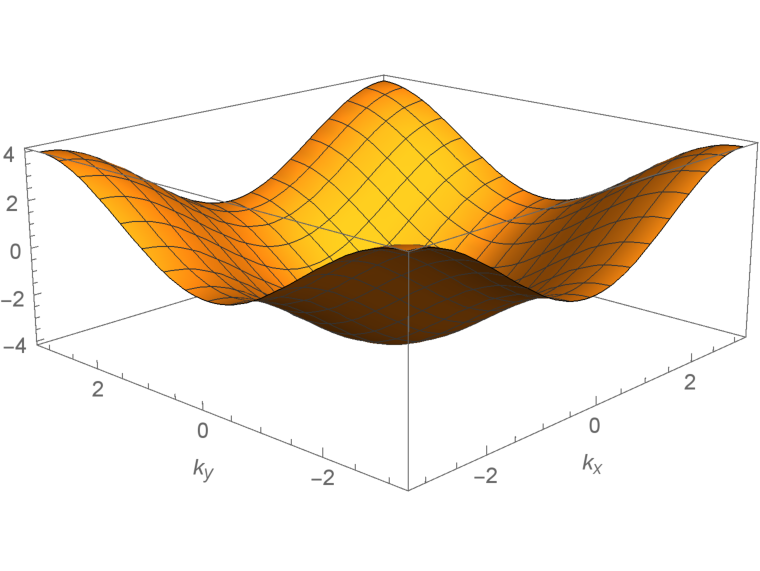
\includegraphics[clip,trim={0 1cm 0 1.2cm},height=6cm, width=6cm, keepaspectratio]{tgsq.pdf}
  \caption{$t > 0$}
  \label{fig:sub1}
\end{subfigure}%
\begin{subfigure}{.5\textwidth}
  \centering
  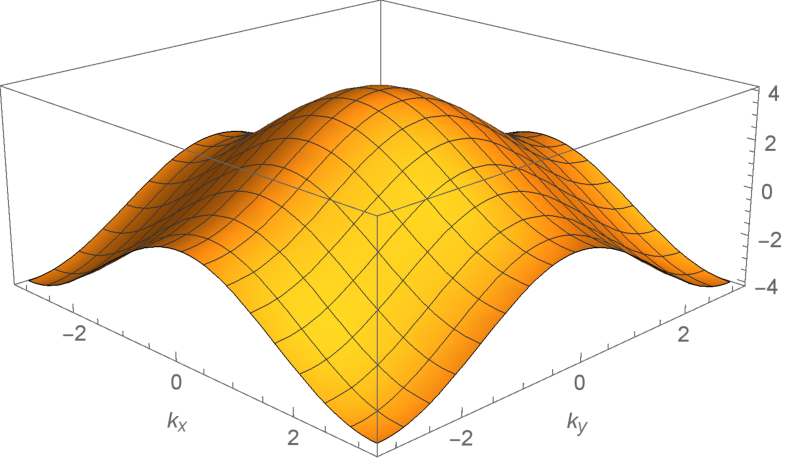
\includegraphics[width= 6cm, height=6cm, keepaspectratio]{tlsq.pdf}
  \caption{$t<0$}
  \label{fig:sub2}
\end{subfigure}
\caption{Dispersion relation for a two-dimensional square lattice}
\label{fig:sq}
\end{figure}

\subsection{Two-dimensional Triangular Lattice}

Following the same procedure as given in the previous section for a two-dimensional triangular lattice, we have,
$$\textbf{R}_\tau = \Big\{(-a,0),(a,0), \Big(\frac{a}{2}, \frac{\sqrt{3}a}{2}\Big), \Big(-\frac{a}{2}, -\frac{\sqrt{3}a}{2}\Big),\Big(-\frac{a}{2}, \frac{\sqrt{3}a}{2}\Big),\Big(\frac{a}{2}, -\frac{\sqrt{3}a}{2}\Big) \Big\} $$
\\
and the energy levels are given by,
\\  
\begin{equation}
\begin{split}
\MoveEqLeft
E_\textbf{k} = -t \big[ e^{-i k_x a} + e^{i k_x a} + e^{i(\frac{a}{2} k_x +\frac{\sqrt{3}a}{2} k_y )}+ e^{i(-\frac{a}{2} k_x -\frac{\sqrt{3}a}{2} k_y )}+ e^{i(-\frac{a}{2} k_x +\frac{\sqrt{3}a}{2} k_y )} +e^{i(\frac{a}{2} k_x -\frac{\sqrt{3}a}{2} k_y )}   \big] \\
& = -2t \Big[cos(k_x a) + cos\Big(\frac{a}{2} k_x +\frac{\sqrt{3}a}{2} k_y\Big)  + cos\Big(\frac{a}{2} k_x -\frac{\sqrt{3}a}{2} k_y\Big)  \Big]
\end{split}
\end{equation}
Again, with $a=1$, for $t>0$, the minimum occurs at  $k_x =0$, $k_y=0$. For $t<0$, the minimum occurs at the four points $k_x = \pm 0.698305 \pi$, $k_y = \pm \pi$. (Figure \ref{fig:tri})

\begin{figure}[h]
\centering
\begin{subfigure}{.5\textwidth}
  \centering
  \adjincludegraphics[height=6cm, width=6cm, keepaspectratio]{tgtri.pdf}
  \caption{$t > 0$}
  \label{fig:sub3}
\end{subfigure}%
\begin{subfigure}{.5\textwidth}
  \centering
  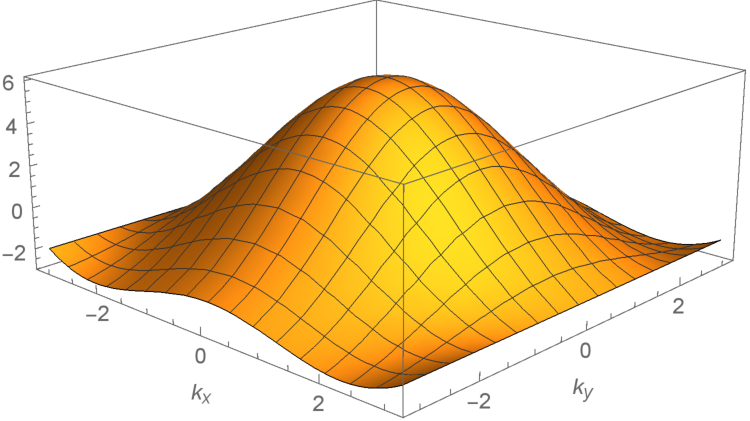
\includegraphics[width= 6cm, height=6.2cm, keepaspectratio]{tltri.pdf}
  \caption{$t<0$}
  \label{fig:sub4}
\end{subfigure}
\caption{Dispersion relation for a two-dimensional triangular lattice}
\label{fig:tri}
\end{figure}

\subsection{Two-dimensional Honeycomb Lattice}

\begin{figure}[H]
\centering
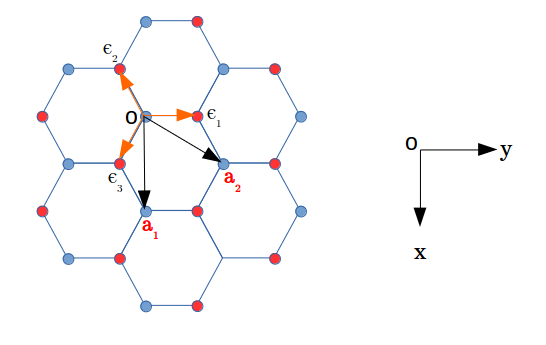
\includegraphics[scale = 0.5]{hc_img_full.png}
\end{figure}

The honeycomb lattice is peculiar in the sense that it is not a Bravais lattice. To find the Bravais lattice for a honeycomb lattice, we need to use the unit cell which contains two neighbouring atoms (one blue atom and one red atom). If we do so, we find that the Bravais lattice for the honeycomb lattice is a hexagonal lattice.
\\\\
The two point basis for this case is as follows: 
\\
\begin{equation}
\textbf{a}_1 = \big(\sqrt{3}a, 0\big), \quad \textbf{a}_2 = \Big(\frac{a}{2}, \frac{\sqrt{3}a}{2}\Big)
\end{equation}
\\
There are three kinds of NN bonds: (1) along y-axis with $\theta = \pi/2$, (2) along $\theta = 7\pi/6$ and (3) along $\theta = 11\pi/6$ and we need to write them separately. The Hamiltonian is be given by,
\begin{equation}
\hat{H} = -t \sum_{i} \big( a_{\textbf{R}_i}^\dagger b_{\textbf{R}_i + \boldsymbol{\epsilon}_1} +  a_{\textbf{R}_i}^\dagger b_{\textbf{R}_i + \boldsymbol{\epsilon}_2} +  a_{\textbf{R}_i}^\dagger b_{\textbf{R}_i + \boldsymbol{\epsilon}_3}\big)  + h.c.
\end{equation}
\\
where, $a_{\textbf{R}_i}^\dagger$ is the creation operator on sublattice-$A$ (blue) and $b_{\textbf{R}_i}$ is the annihilation operator on sublattice-$B$ (red) and $\boldsymbol{\epsilon}_1 = (0,a)$, $\boldsymbol{\epsilon}_2 = \Big(-\frac{\sqrt{3}a}{2}, -\frac{a}{2}\Big)$, $\boldsymbol{\epsilon}_3 = \Big(\frac{\sqrt{3}a}{2}, -\frac{a}{2}\Big)$. Writing the operators in Fourier basis, we have, 

\begin{equation}
a_{\textbf{R}_i}^\dagger = \frac{1}{\sqrt{N}} \sum_{\textbf{k}} a_\textbf{k}^\dagger e^{-i \textbf{k} \cdot \textbf{R}_i}, \quad  \quad  b_{\textbf{R}_i} = \frac{1}{\sqrt{N}} \sum_{\textbf{q}} b_\textbf{q} e^{i \textbf{q} \cdot \textbf{R}_i}
\end{equation}
\\
Hence, the Hamiltonian becomes
\begin{equation}
\begin{split}
\hat{H} & = -t \sum_{\textbf{k}} a_\textbf{k}^\dagger b_\textbf{k} \Big(  e^{i \textbf{k} \cdot \boldsymbol{\epsilon}_1}  + e^{i \textbf{k} \cdot \boldsymbol{\epsilon}_2} + e^{i \textbf{k} \cdot \boldsymbol{\epsilon}_3}\Big)  -t \sum_{\textbf{k}} b_\textbf{k}^\dagger a_\textbf{k}  \Big(  e^{-i \textbf{k} \cdot \boldsymbol{\epsilon}_1}  + e^{-i \textbf{k} \cdot \boldsymbol{\epsilon}_2} + e^{-i \textbf{k} \cdot \boldsymbol{\epsilon}_3}\Big)\\
 & = \sum_{\textbf{k}} \begin{pmatrix} a_\textbf{k}^\dagger & b_\textbf{k}^\dagger \end{pmatrix} \begin{pmatrix} 0 & P(\textbf{k}) \\ Q(\textbf{k}) & 0  \end{pmatrix} \begin{pmatrix} a_\textbf{k} \\ b_\textbf{k} \end{pmatrix}\\
&  = \sum_{\textbf{k}} \Big( a_\textbf{k}^\dagger b_\textbf{k} P(\textbf{k}) + b_\textbf{k}^\dagger a_\textbf{k} Q(\textbf{k}) \Big)
\end{split}
\end{equation}
\\
where $P(\textbf{k}) = -t \Big(  e^{i \textbf{k} \cdot \boldsymbol{\epsilon}_1}  + e^{i \textbf{k} \cdot \boldsymbol{\epsilon}_2} + e^{i \textbf{k} \cdot \boldsymbol{\epsilon}_3}\Big)$ and $Q(\textbf{k}) = P(\textbf{k})^{*}$. Therefore, 

\begin{equation}
\begin{split}
& P(\textbf{k}) = -t \Big[ e^{i k_y a} + 2 e^{-i \frac{a}{2} k_y} cos\Big(\frac{\sqrt{3}ak_x}{2} \Big) \Big] \\
& Q(\textbf{k}) = -t \Big[ e^{-i k_y a} + 2 e^{i \frac{a}{2} k_y} cos\Big(\frac{\sqrt{3}ak_x}{2} \Big) \Big]
\end{split}
\end{equation}
\\
Hence, the kernel of the Hamiltonian is,
\begin{equation}
\hat{H}(\textbf{k}) =  \begin{pmatrix} 0 & P(\textbf{k}) \\ Q(\textbf{k}) & 0  \end{pmatrix} 
\end{equation}
\\
and the eigenvalues of $\hat{H}(\textbf{k}) $ gives the required dispersion relation.

\begin{equation}
\epsilon_{\pm}(\textbf{k}) = \pm \mid P(\textbf{k}) \mid = \pm \mid t \mid \sqrt{3 + 2 cos(\sqrt{3}k_x a) + 4 cos\Big(\frac{\sqrt{3}k_x a}{2} \Big) cos \Big(\frac{\sqrt{3}k_y a}{2} \Big)   }
\end{equation}
\\
Hence, for the honeycomb lattice, we have two different bands which coincide at the corners of the hexagon. (Figure \ref{fig:hc})
\begin{figure}[H]
\centering
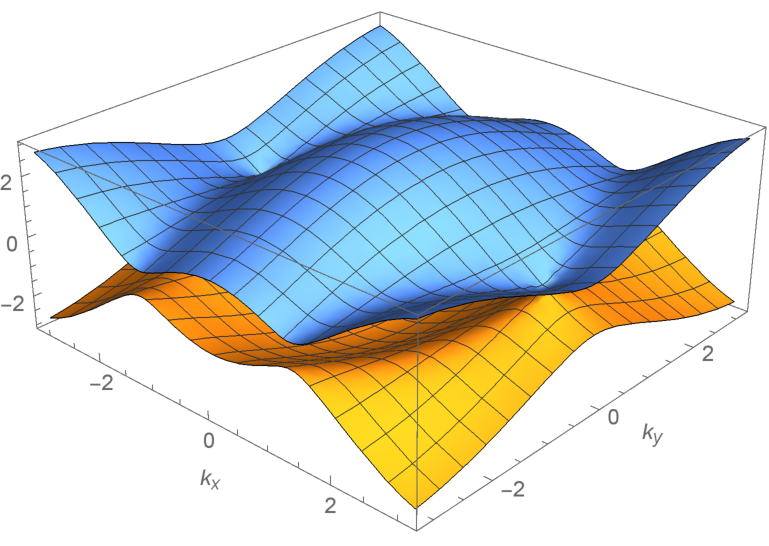
\includegraphics[height=8cm, width = 8cm, keepaspectratio]{hc.pdf}
\caption{Dispersion relation for the two bands of a honeycomb lattice. The two bands coincide at the corners of the hexagon}
\label{fig:hc}
\end{figure}

\section{The Hubbard Model}
The Hubbard model was introduced simultaneously by Gutzwiller, Hubbard and Kanamori. It is the one of the simplest many-body Hamiltonians which allows a meaningful description of two opposing tendencies:

\begin{enumerate}
 \item {the kinetic energy, $\mathcal{H}_{band}$ (electron hopping) delocalizes the electrons into itinerant states, leading to metallic behaviour.}
 \item {the electron-electron interactions, $\mathcal{H}_{U}$, (approximated by Coulomb interaction) localizes the electrons onto sites, with the tendency to  drive the system to an insulating state.}
\end{enumerate}
The usual form of the one-band Hubbard model is given by,
\\
\begin{equation}
\mathcal{H} = \mathcal{H}_{band} + \mathcal{H}_{U} =  -t \sum_{\langle j,l \rangle}\big(c_{j\sigma}^\dagger c_{l\sigma} +   c_{l\sigma}^\dagger c_{j\sigma}\big) + U \sum_{j}\hat{n}_{j \uparrow} \hat{n}_{j \downarrow}
\end{equation}
\\
Here, $-t$ is the tight-binding matrix element for the hopping process and $U$ is the Coulombic repulsion between electrons at the same site. 
\\\\
The operators satisfy the anticommuation relations given by,
\begin{equation}
\begin{split}
&\{c_{j\sigma}, c_{l\sigma ' }^\dagger\} = \delta_{j,l} \delta_{\sigma, \sigma ' }\\
& \{c_{j\sigma}, c_{l\sigma '}\} = 0
\end{split}
\end{equation}
 
\subsection{Classification of Hopping Events}
In the atomic limit ($t=0$), the energy level has huge degeneracy. Every site can be occupied with either $\uparrow$ or $\downarrow$, giving rise to $2^N$ degeneracy at half-filling, where $N$ is the total number of electrons. When a small hopping term $t \ll U$ is switched on, these states are mixed and the sharp atomic level broadens into the lower Hubbard subband. The motion of electrons is restricted by having to avoid the creation of doubly occupied sites. Since, $t \ll U$, we can treat the effect of $\mathcal{H}_{band}$ by perturbation theory. However, on a closer look, this problem is very different from the standard perturbation theory, in which there is a large single-electron term and a weak interaction. In the present case, the zeroth-order term is the interaction term $\mathcal{H}_U$, and the one-electron term is the term $\mathcal{H}_{band}$ is the perturbation. In the standard case, the zeroth-order ground-state is nondegenerate, whereas in this case, $\mathcal{H}_U$ has large degeneracy. Within a degenerate set of levels, even a weak perturbation has a drastic effect; it lifts the degeneracy.
\\\\
This can be systematically dealt with by a suitable $\textit{canonical transformation}$ of the Hamiltonian. The zeroth-order eigenstates are mixed by the perturbation $\mathcal{H}_{band}$. If the ture eigenvalues are known, we could perform a Hilbert-space rotation to that basis, and hence the mixing of states can be avoided. 
\\\\
The hopping processes changes the local configurations. One of the following processes are possible:
\\
\begin{enumerate}
\item  The creation of a doubly occupied site leading to a situation of high-energy state from a low-energy state. This represents a transition from a lower to an upper Hubbard subband. Suppose the hopping takes place from site $i$ which has electron in the $\uparrow$-state before, to site $j$, which becomes $d$-state after the hopping, the related $\textit{projected hopping term}$ is
\\
\begin{equation}
\hat{P}_{jd}c_{j\uparrow}^\dagger c_{i\uparrow} \hat{P}_{i\uparrow} = \hat{n}_{j\uparrow} \hat{n}_{j\downarrow} c_{j\uparrow}^\dagger c_{i\uparrow} \hat{n}_{i\uparrow} (1 - \hat{n}_{i\downarrow}) = \hat{n}_{j\downarrow} c_{j\uparrow}^\dagger c_{i\uparrow}(1 - \hat{n}_{i\downarrow}) 
\end{equation}

Collecting all the similar contributions, the Hamiltonian operator of hopping processes which increase the number of doubly occupied sites by one, can be given by,

\begin{equation}
\mathcal{H}_{t}^{+} = -t \sum_{\langle i, j \rangle} \sum_{\sigma} \big[\hat{n}_{i-\sigma} c_{i\sigma}^\dagger c_{j\sigma}(1 - \hat{n}_{j-\sigma})   + \hat{n}_{j-\sigma} c_{j\sigma}^\dagger c_{i\sigma}(1 - \hat{n}_{i-\sigma})  \big]
\end{equation} 

\item Similarly, the Hamiltonian operator of hopping processes that decrease the doubly occupied sites by one, is given by,
\begin{equation}
\mathcal{H}_{t}^{-} = -t \sum_{\langle i, j \rangle} \sum_{\sigma} \big[(1-\hat{n}_{i-\sigma}) c_{i\sigma}^\dagger c_{j\sigma}\hat{n}_{j\sigma}   + (1-\hat{n}_{j-\sigma}) c_{j\sigma}^\dagger c_{i\sigma}\hat{n}_{i\sigma}  \big]
\end{equation}

\item 
There are also processes that do not change the total number of doubly occupied sites. Firstly, it is possible that there is no doubly occupied site to begin with, and it is also not created after the hopping takes place. In this process, the electron remains in the lower Hubbard subband. Another possibility is that it starts out, and remains in the upper Hubbard subband. These two processes can be mathematically written as,

\begin{equation}
\mathcal{H}_{t}^{0} = -t \sum_{\langle i, j \rangle} \sum_{\sigma} \big[(1-\hat{n}_{i-\sigma}) c_{i\sigma}^\dagger c_{j\sigma}(1-\hat{n}_{j-\sigma})   + \hat{n}_{i-\sigma} c_{i\sigma}^\dagger c_{j\sigma}\hat{n}_{i-\sigma} + H.c.  \big]
\end{equation}

\end{enumerate} 
Since we have enumerated all the possible types of hopping events, the kinetic energy term can be decomposed into three terms,

\begin{equation}
\mathcal{H}_{band} = \mathcal{H}_{t}^{+} + \mathcal{H}_{t}^{-}+ \mathcal{H}_{t}^{0}
\end{equation}

\subsection{The Canonical Transformation}

The kinetic energy part of the Hamiltonian $\mathcal{H}_{band}$ mixes the states from the two Hubbard subbands via the terms  $\mathcal{H}_{t}^{+}$ and $\mathcal{H}_{t}^{-}$. A rotation (in the many-electron Hilbert space) to a suitable linear combination of the uncorrelated basis states is achieved by a canonical transformation. In this new basis, the Hubbard Hamiltonian,
\\
\begin{equation}
\mathcal{H} = \mathcal{H}_{t}^{+} + \mathcal{H}_{t}^{-}+ \mathcal{H}_{t}^{0} + \mathcal{H}_{U}
\end{equation} 
\\
acts like the \textit{effective Hamiltonian},
\\
\begin{equation}
\begin{split}
\mathcal{H}_{\texttt{eff}} =  & e^{iS} \mathcal{H} e^{-iS} = \mathcal{H} + i[S, \mathcal{H}] + \frac{i^2}{2} [S, [S,\mathcal{H}]] + ...\\
=  & \mathcal{H}_U + \mathcal{H}_{t}^{+} + \mathcal{H}_{t}^{-} + \mathcal{H}_{t}^{0} + i[S, \mathcal{H}_U]\\
   &+ i[S, \mathcal{H}_{t}^{+} + \mathcal{H}_{t}^{-}+ \mathcal{H}_{t}^{0}] + \frac{i^2}{2} [S, [S,\mathcal{H}]] + ...
\end{split}
\end{equation}
\\
The generator $S$ must be chosen in such a way that $\mathcal{H}_{\texttt{eff}}$ doesn't connect different subbands. Firstly, we will eliminate the largest cross-terms, $\mathcal{H}_{t}^{+} + \mathcal{H}_{t}^{-}$ which are of the order $t$. Since the largest term of $i[S, \mathcal{H}] $ is $i[S, \mathcal{H}_U] $, we must require that this cancels with $\mathcal{H}_{t}^{+} + \mathcal{H}_{t}^{-}$. It follows that $S$ must be of the order of $t/U$, from which we obtain, 
\\
\begin{equation}
[\mathcal{H}_{t}^{+}, \mathcal{H}_U] = -U\mathcal{H}_{t}^{+},  \quad \quad \quad  [\mathcal{H}_{t}^{-}, \mathcal{H}_U] = U\mathcal{H}_{t}^{-}
\end{equation}
\\
Hence, we must use 
\\
\begin{equation}
S = -\frac{i}{U} (\mathcal{H}_{t}^{+} - \mathcal{H}_{t}^{-})
\end{equation}
\\
because
\\
\begin{equation}
i[S, \mathcal{H}_U] = \frac{1}{U}[\mathcal{H}_{t}^{+} - \mathcal{H}_{t}^{-}, \mathcal{H}_U ] = -(\mathcal{H}_{t}^{+} - \mathcal{H}_{t}^{-})
\end{equation}
\\
cancels the unwanted part of $\mathcal{H}_{band}$. However, we also generate new terms of the form
\\
\begin{equation}
i[S, \mathcal{H}_{t}^{+} + \mathcal{H}_{t}^{-}] =  \frac{1}{U} [\mathcal{H}_{t}^{+} - \mathcal{H}_{t}^{-},\mathcal{H}_{t}^{+} + \mathcal{H}_{t}^{-}] = \frac{2}{U} [\mathcal{H}_{t}^{+}, \mathcal{H}_{t}^{-}]
\end{equation}
\\
which is of the order of $t^2/U$. We also have the term following term which provides a contribution of the same order of magnitude
\\
\begin{equation}
\frac{i^2}{2}[S, [S,\mathcal{H}_{U}]] = -\frac{i}{2}[S, \mathcal{H}_{t}^{+} + \mathcal{H}_{t}^{-}] = -\frac{1}{U} [\mathcal{H}_{t}^{+}, \mathcal{H}_{t}^{-}]
\end{equation}
\\
Combining the above two equations and omitting the contributions coming from the $i[S, \mathcal{H}_{t}^0]$, the effective Hamiltonian (to order $t^2/U$) is found to be 
\\ 
\begin{equation}
\mathcal{H}_{\texttt{eff}} = \mathcal{H}_{t}^0 + \mathcal{H}_{U} + \frac{1}{U} [\mathcal{H}_{t}^{+}, \mathcal{H}_{t}^{-}]
\end{equation}

\subsection{The \textit{t - J} Model}
The $\mathcal{H}_{t}^{+}$ and $\mathcal{H}_{t}^{-}$ are the sums of pair operators. We knnow that operations at disjoint pairs commute, non-vanishing contributions arise only if the pairs have one or two sites in common. The commutator can thus be written as:
\\
\begin{equation}
[\mathcal{H}_{t}^{+}, \mathcal{H}_{t}^{-}] = \sum_{\langle i,j \rangle}\sum_{\langle k, l \rangle} [\mathcal{H}_{t, ij}^{+}, \mathcal{H}_{t, kl}^{-}] =    \sum_{\langle i,j \rangle} [\mathcal{H}_{t, ij}^{+}, \mathcal{H}_{t, ij}^{-}] + \sum_{\langle i,j,k \rangle} [\mathcal{H}_{t, ij}^{+}, \mathcal{H}_{t, jk}^{-}]
\end{equation}
\\
Upon solving, for a jump from site $j$ to site $i$, we obtain,
\\
\begin{equation}
\frac{1}{U} [\mathcal{H}_{t, ij}^{+}, \mathcal{H}_{t, ij}^{-}] = \frac{2t^2}{U} \Big(\textbf{S}_i \cdot \textbf{S}_j - \frac{\hat{n}_i \hat{n}_j}{4} \Big)
\end{equation} 
\\
The same contribution is also obtained if the jump is from  $i$ to $j$. Hence, we obtain the $\mathcal{H}_{\texttt{eff}}$ or the Hamiltonian for the \textit{t -J model}.
\\
\begin{equation}
\mathcal{H}_{\texttt{eff}} \equiv \mathcal{H}_{tJ} = \mathcal{H}_t^0 +  \frac{4t^2}{U}\sum_{\langle i,j \rangle} \Big(\textbf{S}_i \cdot \textbf{S}_j - \frac{\hat{n}_i \hat{n}_j}{4} \Big) + \texttt{three site terms}
\end{equation}
\\

\section{The Kondo Lattice}


The simplest Kondo Lattice Hamiltonian with an $s$-wave form factor is 
\\
\begin{equation}
\mathcal{H}_{\textsf{KL}} = \sum_{\textbf{k}\sigma} \epsilon_{\textbf{k}} c_{\textbf{k}\sigma}^\dagger c_{\textbf{k}\sigma} + \frac{J}{2} \sum_{j}\sum_{\alpha \beta} \textbf{S}_{j} \cdot \big(c_{j\alpha}^\dagger \vec{\sigma}_{\alpha \beta} c_{j\beta}\big)
\end{equation}
\\
where $\vec{\sigma}$ is the vector of Pauli matrices and the Kondo coupling $J$ is antiferromagnetic. 

\subsection{Indirect Exchange}
The local $\textit{f-c}$ exchange polarizes the surrounding Fermi sea which carries this information to the other $\textit{f}$-sites, mediating an effective $\textit{f}$-spin--$\textit{f}$-spin interaction. Let us pick out two $\textit{f}$-shells, situated at $\textbf{R}_1$ and $\textbf{R}_2$, which bear the spins $\textbf{S}_1$ and $\textbf{S}_2$, respectively. We will consider the two-step process in which a spin-flip scattering at site $\textbf{R}_1$ is followed by a spin-flip scattering at site $\textbf{R}_2$ 
\\
\begin{figure}[H]
\centering
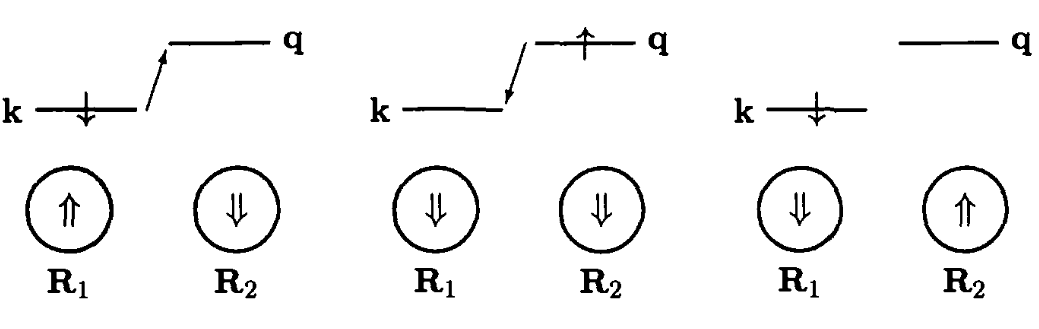
\includegraphics[scale=0.35]{scattering.png}
\end{figure}

This problem can be conveniently tackled by performing a canonical transformation on the Kondo lattice model. The Kondo lattice Hamiltonian can be considered as
\\
\begin{equation}
\mathcal{H} = \mathcal{H}_{0} + \mathcal{H}_{1}
\end{equation}
\\
where
\\
\begin{equation}
 \mathcal{H}_{1}= \frac{J}{2L}\sum_{j=1}^{2}e^{i(\textbf{k}-\textbf{q}) \cdot \textbf{R}_j} \textbf{S}_j \cdot \Bigg(\sum_{\alpha, \beta} c_{\textbf{q}\sigma}^\dagger \vec{\sigma}_{\alpha \beta} c_{\textbf{k}\sigma}\Bigg)
\end{equation}
\\
Upon transforming the $f-c$ interactions, the effective Hamiltonian will contain the required $f-f$ interactions. 
\\
\begin{equation}
\mathcal{H}_{\texttt{eff}} = e^{iS} \mathcal{H} e^{-iS} \approx \mathcal{H} + [iS, \mathcal{H}] + \frac{1}{2}[iS, [iS, \mathcal{H}]]
\end{equation}
\\
We want 
\\
\begin{equation}\label{eq:S}
\mathcal{H}_{1} + [iS, \mathcal{H}_0] = 0
\end{equation}
\\
which gives
\\
\begin{equation}
\mathcal{H}_{\texttt{eff}} = \mathcal{H}_0 + \frac{1}{2}[iS, \mathcal{H}_1]
\end{equation}
\\
It can be checked that Equation (\ref{eq:S}) is satisfied by 
\\
\begin{equation}
iS = \frac{J}{2L}\sum_{j=1}^{2}\sum_{\textbf{k}, \textbf{q}} \frac{e^{i(\textbf{k}-\textbf{q}) \cdot \textbf{R}_j}}{\epsilon_{\textbf{k}} - \epsilon_{\textbf{q}}} \Big[ S_j^+ c_{\textbf{k}\downarrow}^\dagger c_{\textbf{q}\uparrow} + S_j^- c_{\textbf{k}\uparrow}^\dagger c_{\textbf{q}\downarrow} + S_j^z \big( c_{\textbf{k}\uparrow}^\dagger c_{\textbf{q}\uparrow} - c_{\textbf{k}\downarrow}^\dagger c_{\textbf{q}\downarrow}\big)\Big]
\end{equation}
\\
On evaluating the commutator and collecting all the relevant terms, the interaction seems to be isotropic, i.e., proportional to $\textbf{S}_i \cdot \textbf{S}_j$. The same kind of interaction term can be derived for an arbitrary pair of sites and thus for a periodic lattice, the effective Hamiltonian can be written as the sum of conduction band kinetic energy and the indirect exchange interaction
\\
\begin{equation}
\mathcal{H}_{\textsf{RKKY}} = \sum_{\textbf{k}\sigma} \epsilon_{\textbf{k}}\hat{n}_{\textbf{k}\sigma} + \frac{1}{2} \sum_{i \neq j} \mathcal{I}(\textbf{R}_i - \textbf{R}_j) \textbf{S}_i \cdot \textbf{S}_j
\end{equation}
\\
where the coupling strength of the Ruderman-Kittel-Kasuya-Yosida (RKKY) interaction is 
\\
\begin{equation}
\mathcal{I}(\textbf{R}_i - \textbf{R}_j) = - J^2 \sum_{\textbf{k}, \textbf{q}}cos\big[(\textbf{k}-\textbf{q})(\textbf{R}_i-\textbf{R}_j)\big]  \frac{f_\textbf{k} - f_\textbf{q}}{\epsilon_{\textbf{q}} - \epsilon_{\textbf{k}}}
\end{equation}

\subsection{Solving for the Three-dimensional Lattice}
This can be further evaluated using the free-electron dispersion relation $\epsilon_\textbf{k} = \hbar^2 k^2 /2m$. Rewriting the cosines as exponentials and using $\textbf{R} = \textbf{R}_i - \textbf{R}_j$,  $\theta$ being the angle subtended by $\textbf{q}$ and $\textbf{R}$, we have integrals like (which can be evaluated using the contour integral techniques)
\\
\begin{equation}
\int d\textbf{q} \frac{e^{i \textbf{q} \cdot \textbf{R}}}{q^2 - k^2} = 2\pi \int_{0}^{\infty}q^2 dq \int_{0}^{\pi} d\theta \sin\theta\frac{e^{iqR \cos\theta}}{q^2 - k^2} = \frac{4\pi^2}{R} \cos(kR)
\end{equation}
\\
Hence, we have the following
\\
\begin{equation}
\begin{split}
\mathcal{I}_{\textsf{3D}}(\textbf{R}_i - \textbf{R}_j) &= -J^2 \Bigg(\frac{m}{2\hbar^2}\Bigg)\Bigg[ \sum_{k} \frac{2\pi^2}{R} \cos(kR)e^{-i\textbf{k} \cdot \textbf{R}} + \sum_{k} \frac{2\pi^2}{R} \cos(kR)e^{i\textbf{k} \cdot \textbf{R}}  \Bigg]\\
&= -J^2 \Bigg(\frac{m}{\hbar^2}\Bigg) \sum_{k} \frac{2\pi^2}{R} \cos(kR) \cos(\textbf{k} \cdot \textbf{R})\\
&=  -J^2 \Bigg(\frac{2m\pi^2}{\hbar^2 R}  \Bigg) \frac{4\pi}{R} \int_{0}^{k_F} kdk \cos(kR) \sin(kR)
\end{split}
\end{equation}
\\
Now, upon solving the \textbf{k}-integral, we have the following
\\
\begin{equation}
\begin{split}
\mathcal{I}_{\textsf{3D}}(\textbf{R}_i - \textbf{R}_j) &= -J^2 \Bigg(\frac{\pi^3m}{\hbar^2 R^4}\Bigg) \big[\sin(2k_F R_{ij}) - 2k_F R_{ij}\cos(2k_F R_{ij})\big]\\
&= -J^2 \Bigg(\frac{16\pi^3 m k_F^4}{\hbar^2}\Bigg) \frac{\sin(2k_F R_{ij}) - 2k_F R_{ij} \cos(2k_F R_{ij})}{(2k_F R_{ij})^4}
\end{split}
\end{equation}
\\
where $R_{ij} =  \mid\textbf{R}_i - \textbf{R}_j \mid$. Hence, in 3D, the RKKY interaction oscillates and it is long-ranged as it decays according to a power law.
 
\subsection{Solving for the Two-dimensional Lattice}
Considering the similar integrals as in the previous section, for a two-dimensional lattice, we have
\\
\begin{equation}\label{eq:bessel}
\int d\textbf{q} \frac{e^{i \textbf{q} \cdot \textbf{R}}}{q^2 - k^2} =  \int_{0}^{\infty}\frac{q dq}{q^2-k^2} \int_{0}^{2\pi}e^{iqR \cos\theta}d\theta 
\end{equation} 
\\
The $\theta$-integral gives the Bessel function of first kind and zeroth order, $J_0$. 
\begin{equation}
\int_{0}^{2\pi}e^{iqR \cos\theta}d\theta = 2\pi J_0(qR)
\end{equation}
\\
Putting this back in Equation (\ref{eq:bessel}), we have
\\
\begin{equation}
2\pi\int_{0}^{\infty}\frac{q dq}{q^2-k^2} J_0(qR) = 2\pi \Big( -\frac{\pi}{2} Y_0(qR) \Big) = -\pi^2 Y_0(kR)
\end{equation}
\\
where  $Y_0$ is the Bessel function of second kind and zeroth order. Hence, we have the following
\\
\begin{equation}
\begin{split}
\mathcal{I}_{\textsf{2D}}(\textbf{R}_i - \textbf{R}_j) &= -J^2 \Bigg(\frac{m}{2\hbar^2}\Bigg)\Big[-\frac{\pi^2}{2}\sum_{k}Y_0(kR)e^{-i\textbf{k} \cdot \textbf{R}}    -\frac{\pi^2}{2} \sum_{k}Y_0(kR)e^{i\textbf{k} \cdot \textbf{R}}  \Big]\\
&= J^2 \Bigg(\frac{m\pi^2}{2\hbar^2}\Bigg)\Bigg[\int_{0}^{k_F}k dk Y_0(kR) \int_{0}^{2\pi}e^{ikR \cos\theta}d\theta \Bigg]\\
&= J^2 \Bigg(\frac{m\pi^2}{2\hbar^2}\Bigg) 2\pi \int_{0}^{k_F}k dk Y_0(kR)J_0(kR)
\end{split}
\end{equation}
\\
Using the integral relation 
\\
\begin{equation}
\int_{0}^{a} x  J_0(x) Y_0(x)dx = \frac{a^2}{2}\Big(J_0(a) Y_0(a) +  J_1(a) Y_1(a)  \Big)
\end{equation}
\\
where $J_1$ and $Y_1$ are the Bessel functions of first order of first and second kinds respectively, we finally have the RKKY interaction in a 2D lattice.
\\
\begin{equation}
\mathcal{I}_{\textsf{2D}}(\textbf{R}_i - \textbf{R}_j) = J^2 \Bigg(\frac{ \pi^3mk_F^2}{2\hbar^2 }\Bigg)\Big(J_0(k_F R_{ij}) Y_0(k_F R_{ij}) +  J_1(k_F R_{ij}) Y_1(k_F R_{ij}) \Big)
\end{equation}

\subsection{Solving for the One-dimensional Lattice}
In the one-dimensional case, the integrals are rather simpler. We have the following integral
\\
\begin{equation}
\begin{split}
\int d\textbf{q} \frac{e^{i \textbf{q} \cdot \textbf{R}}}{q^2 - k^2} & = \int_{0}^{\infty} dq \frac{e^{i qR}}{q^2 - k^2}  + \int_{0}^{\infty} dq \frac{e^{-i qR}}{q^2 - k^2} = \int_{-\infty}^{\infty} dq \frac{e^{i qR}}{q^2 - k^2}\\
& = -\frac{2\pi}{k} \sin(kR)
\end{split}
\end{equation}
\\
Therefore, the interaction term becomes
\\
\begin{equation}
\begin{split}
\mathcal{I}_{\textsf{1D}}(\textbf{R}_i - \textbf{R}_j) & = -J^2 \Bigg(\frac{m}{2\hbar^2} \Bigg)\Bigg[-\pi\sum_{k} \frac{ \sin(kR)}{k}e^{-i\textbf{k} \cdot \textbf{R}}    + -\pi\sum_{k} \frac{sin(kR)}{k}e^{i\textbf{k} \cdot \textbf{R}}\Bigg]\\
& = J^2 \Bigg(\frac{m\pi}{\hbar^2} \Bigg) \sum_{k}\frac{\sin(kR)\cos(\textbf{k} \cdot \textbf{R})}{k}\\
& = J^2 \Bigg(\frac{2m\pi}{\hbar^2} \Bigg) \sum_{k}\frac{\sin(kR)\cos(kR)}{k}\\
& = J^2 \Bigg(\frac{m\pi}{\hbar^2} \Bigg)\sum_{k}\frac{\sin(2kR)}{k}
\end{split}
\end{equation}
\\
Now. performing the $\textbf{k}$-integral, we note that
\\
\begin{equation}
\int_{0}^{a} \frac{\sin(x)}{x} = Si(a)
\end{equation}
\\
where, $Si$ is the Sine integral function. Hence, the interaction becomes
\\
\begin{equation}
\mathcal{I}_{\textsf{1D}}(\textbf{R}_i - \textbf{R}_j) = J^2 \Bigg(\frac{m\pi}{\hbar^2}\Bigg) Si(2k_FR_{ij})
\end{equation} 
\\
But, due to a peculiar non-analyticity at $\textbf{k}=0$, $\textbf{q}=0$, the order of integral cannot be reversed and the integral over \textbf{k} should be performed first. As a result, the correct solution is obtained by replacing $Si(2k_FR_{ij})$ with $Si(2k_FR_{ij}) - \pi/2$. Hence, the RKKY interaction in 1D is given by
\\
\begin{equation}
\mathcal{I}_{\textsf{1D}}(\textbf{R}_i - \textbf{R}_j) = -J^2 \Bigg(\frac{m\pi}{\hbar^2}\Bigg)\Bigg(\frac{\pi}{2} - Si(2k_FR_{ij})\Bigg)
\end{equation}

\section{Using the p-Wave Form Factor in Kondo Lattice}
In the previous section, we saw the RKKY Interaction in 3D, 2D and 1D for an $s$-wave form factor. The same procedure can be carried out by plugging in the p-wave form factor into the Kondo lattice Hamiltonian. 
\\\\
The new Hamiltonian with p-wave form factor looks like
\\
\begin{equation}
\mathcal{H}_{\textsf{KL}} = \sum_{\textbf{k}\sigma} \epsilon_{\textbf{k}} c_{\textbf{k}\sigma}^\dagger c_{\textbf{k}\sigma} + \frac{J}{2} \sum_{j}\sum_{\alpha \beta} \textbf{S}_{j} \cdot \big(\Psi_{j\alpha}^\dagger \vec{\sigma}_{\alpha \beta} \Psi_{j\beta}\big)
\end{equation}
\\
where
\\
\begin{equation}
\Psi_{j\alpha} = \sum_{l, \beta} \Phi_{jl}^{\alpha \beta} c_{j \beta}
\end{equation}
\\
and
\\

\begin{equation}
 \Phi_{ij}^{\alpha \beta} (\hat{\textbf{R}}) = 
 \begin{cases}
 \centering
- i\hat{\textbf{R}} \cdot \Big( \frac{\vec{\sigma}}{2} \Big), & \text{if }i,j\text{ are nearest neighbours} \\
 0, & \text{otherwise}
\end{cases}
\end{equation}
\\

\subsection{The One-dimensional Case}
Putting the values of $\Psi_{j\alpha}^\dagger$ and $\Psi_{j\beta}$ for a 1D case and assuming the lattice to lie along the $z$-axis, we have
\\
\begin{equation}
\begin{split}
\mathcal{H}_1 &=  \frac{J}{8} \sum_{j}\sum_{\alpha \beta} \textbf{S}_{j} \cdot \big\{ [c_{j+1, \alpha}^\dagger -  c_{j-1, \alpha}^\dagger] \sigma_z \vec{\sigma}_{\alpha \beta} \sigma_z [c_{j+1, \beta} -  c_{j-1, \beta}] \big\}\\
&= \frac{J}{8} \sum_{j}\sum_{\alpha \beta} \textbf{S}_{j} \cdot \big\{ [c_{j+1, \alpha}^\dagger -  c_{j-1, \alpha}^\dagger]  \tilde{\sigma}            [c_{j+1, \beta} -  c_{j-1, \beta}] \big\}
\end{split}
\end{equation}
\\
where $\tilde{\sigma}\equiv \sigma_z \vec{\sigma}_{\alpha \beta} \sigma_z= (-\sigma_x, -\sigma_y, \sigma_z)$. Representing the above equation in the Fourier basis, we obtain
\\
\begin{equation}
\begin{split}
\mathcal{H}_1 &= \frac{J}{8} \sum_{j}\sum_{\alpha \beta} \textbf{S}_{j} \cdot \Bigg\{ \sum_{\textbf{q}}\Big[ e^{-i\textbf{q} \cdot \textbf{R}_{j+1}} - e^{-i\textbf{q} \cdot \textbf{R}_{j-1}}   \Big] c_{\textbf{q},\alpha}^\dagger \tilde{\sigma}c_{\textbf{k},\beta} \sum_{\textbf{k}} \Big[ e^{i\textbf{k} \cdot \textbf{R}_{j+1}} - e^{i\textbf{k} \cdot \textbf{R}_{j-1}}   \Big] \Bigg\}\\
&= \frac{J}{8} \sum_{j}\sum_{\alpha \beta}  \sum_{\textbf{q},\textbf{k}} e^{i(\textbf{k}-\textbf{q}) \cdot\textbf{R}_j} \textbf{S}_{j} \cdot \Bigg\{\Big[ e^{-iqa} - e^{iqa}   \Big] c_{\textbf{q},\alpha}^\dagger \tilde{\sigma}c_{\textbf{k},\beta}  \Big[ e^{ika} - e^{-ika}   \Big] \Bigg\}\\
&= \frac{J}{2} \sum_{j}\sum_{\alpha \beta}\sum_{\textbf{q}, \textbf{k}}e^{i(\textbf{k}-\textbf{q}) \cdot\textbf{R}_j} \sin(qa)\sin(ka) \textbf{S}_{j} \cdot \Big\{ c_{\textbf{q},\alpha}^\dagger \tilde{\sigma}c_{\textbf{k},\beta}   \Big\}\\
\end{split}
\end{equation}
\\
Summing over $\alpha$, $\beta$ and representing the expression as before, we have
\\
\begin{equation}
\mathcal{H}_1 = \frac{J}{2} \sum_{j}\sum_{\textbf{q}, \textbf{k}}e^{i(\textbf{k}-\textbf{q}) \cdot\textbf{R}_j} \sin(qa) \sin(ka)\Big[ -S_j^+ c_{\textbf{q}\downarrow}^\dagger c_{\textbf{k}\uparrow} - S_j^- c_{\textbf{q}\uparrow}^\dagger c_{\textbf{k}\downarrow} + S_j^z \big( c_{\textbf{q}\uparrow}^\dagger c_{\textbf{k}\uparrow} - c_{\textbf{q}\downarrow}^\dagger c_{\textbf{k}\downarrow}\big)\Big]
\end{equation}
Similarly, the $iS$ that would satisfy the relation $[iS, \mathcal{H}_0] = -\mathcal{H}_1$ is 
\\
\begin{equation}
iS = \frac{J}{2} \sum_{j}\sum_{\textbf{q}, \textbf{k}}\frac{e^{i(\textbf{k}-\textbf{q}) \cdot\textbf{R}_j}}{\epsilon_\textbf{q} - \epsilon_\textbf{k}} \sin(qa)\sin(ka)\Big[ -S_j^+ c_{\textbf{q}\downarrow}^\dagger c_{\textbf{k}\uparrow} - S_j^- c_{\textbf{q}\uparrow}^\dagger c_{\textbf{k}\downarrow} + S_j^z \big( c_{\textbf{q}\uparrow}^\dagger c_{\textbf{k}\uparrow} - c_{\textbf{q}\downarrow}^\dagger c_{\textbf{k}\downarrow}\big)\Big]
\end{equation}
\\
Using the similar procedure as in the previous section, we can solve for the effective Hamiltonian, and the interaction term becomes
\\
\begin{equation}
\mathcal{I}_{\textsf{p-wave, 1D}}(\textbf{R}_i - \textbf{R}_j)  =  \Bigg(\frac{J}{2}\Bigg)^2 \sum_{\textbf{q}, \textbf{k}} \cos[(\textbf{k}-\textbf{q})\cdot(\textbf{R}_i - \textbf{R}_j)] \sin^{2}(qa) \sin^{2}(ka) \frac{f_\textbf{k} - f_\textbf{q}}{\epsilon_\textbf{q} - \epsilon_\textbf{k} }
\end{equation} 
\\
Upon solving, it is seen that the above interaction function is a step function and assumes different functional values for $R > 2a$ and $R < 2a$, where $R = |\textbf{R}_i - \textbf{R}_j|$.
\\
\begin{equation}
\mathcal{I}_{\textsf{p-wave, 1D}}(\textbf{R}_i - \textbf{R}_j) =
\begin{cases}
\centering
\begin{split}
\bigg(\frac{J}{2}\bigg)^2 \frac{m \pi}{8 \hbar^2} &\Big[ 4Sin(2k_fa) - 2Si(4k_fa) - 4Si(2k_fR) \\ &+ 4Si(2k_f(R+a)) - Si(2k_f(R+2a)) +Si(2k_f(R-2a))\Big]
 \end{split}  & , R < 2a    \\

\begin{split}
\bigg(\frac{J}{2}\bigg)^2 \frac{m \pi}{8 \hbar^2} &\Big[ 4Sin(2k_f(R-a)) + 4Si(2k_f(R+a)) - Si(2k_f(R+2a)) \\ & - Si(2k_f(R-2a)) -6Si(2k_fR)\Big]
\end{split}  & , R > 2a\\
\end{cases}
\end{equation}
\\
A similar calculation can be carried out for a system of ``\textit{extended s-wave}", where ***. For the extended s-wave system, the interaction term can be given by
\\
\begin{equation}
\mathcal{I}_{\textsf{ext s-wave, 1D}}(\textbf{R}_i - \textbf{R}_j)  =  \Bigg(\frac{J}{2}\Bigg)^2 \sum_{\textbf{q}, \textbf{k}} \cos[(\textbf{k}-\textbf{q})\cdot(\textbf{R}_i - \textbf{R}_j)] \cos^{2}(qa) \cos^{2}(ka) \frac{f_\textbf{k} - f_\textbf{q}}{\epsilon_\textbf{q} - \epsilon_\textbf{k} }
\end{equation}
\\
Upon solving the above expression further, we find that interaction function is again a step function, splitting at $R = 2a$. The results for extended s-wave are
\\
\begin{equation}
\mathcal{I}_{\textsf{p-wave, 1D}}(\textbf{R}_i - \textbf{R}_j) =
\begin{cases}
\centering
\begin{split}
\bigg(\frac{J}{2}\bigg)^2 \frac{m \pi}{8 \hbar^2} &\Big[ -4Si(2k_fa) -2Si(4k_fa) -4Si(2k_fR) \\ & -4Si(2k_f(R+a)) - Si(2k_f(R+2a)) +Si(2k_f(R-2a))\Big]
 \end{split}  & , R < 2a    \\

\begin{split}
\bigg(\frac{J}{2}\bigg)^2 \frac{m \pi}{8 \hbar^2} &\Big[ -4Si(2k_f(R-a)) -6Si(2k_fR) -4Si(2k_f(R+a)) \\ & - Si(2k_f(R+2a)) -Si(2k_f(R-2a))\Big]
\end{split}  & , R > 2a\\
\end{cases} 
\end{equation}





\subsection{The Three-dimensional Case}
Performing the calculation for the three dimensional case with the \textit{p}-wave form factor is quite tricky and cumbersome, since we get a lot of terms while evaluating the commutators, hence we tried to find a general solution.
The $\mathcal{H}_1$ for three-dimension after expansion in the Fourier basis becomes
\\
\begin{equation}
\mathcal{H}_1 =  \frac{J}{2} \sum_{j} \sum_{\alpha, \beta} \sum_{\textbf{q}, \textbf{k}} e^{i(\textbf{k} - \textbf{q}) \cdot \textbf{R}_j} \textbf{S}_j \cdot \Big(A_\textbf{q} c_{\textbf{q}, \alpha}^\dagger \vec{\sigma}_{\alpha \beta} c_{\textbf{k}, \beta} A_\textbf{k} \Big)
\end{equation}
\\
where $A_\textbf{q} \equiv \sin(q_xa) \sigma_x + \sin(q_ya) \sigma_y + \sin(q_za) \sigma_z$ and $A_\textbf{k} \equiv \sin(k_xa) \sigma_x + \sin(k_ya) \sigma_y + \sin(k_za) \sigma_z$. Similarly, $iS$ can be given by
\\
\begin{equation}
iS = \frac{J}{2} \sum_{j} \sum_{\alpha, \beta} \sum_{\textbf{q}, \textbf{k}} \frac{e^{i(\textbf{k} - \textbf{q}) \cdot \textbf{R}_j}}{\epsilon_{\textbf{q}} - \epsilon_{\textbf{k}}} \textbf{S}_j \cdot \Big(  A_\textbf{q} c_{\textbf{q}, \alpha}^\dagger \vec{\sigma}_{\alpha \beta} c_{\textbf{k}, \beta} A_\textbf{k} \Big)
\end{equation}
\\
In the commutator $[iS, \mathcal{H}_1]$, we will have terms like
\\
\begin{multline}
[S_1^x c_{\textbf{q}}^\dagger A_{\textbf{q}} \sigma_x A_{\textbf{k}} c_\textbf{k},  S_2^xc_{\textbf{k}}^\dagger A_{\textbf{k}} \sigma_x A_{\textbf{q}} c_\textbf{q}] =  S_1^xS_2^xc_{\textbf{q}}^\dagger A_{\textbf{q}} \sigma_x A_{\textbf{k}} c_\textbf{k}c_{\textbf{k}}^\dagger A_{\textbf{k}} \sigma_x A_{\textbf{q}} c_\textbf{q}  - S_1^xS_2^x c_{\textbf{k}}^\dagger A_{\textbf{k}} \sigma_x A_{\textbf{q}} c_\textbf{q}  c_{\textbf{q}}^\dagger A_{\textbf{q}} \sigma_x A_{\textbf{k}} c_\textbf{k}\\
\quad
= S_1^xS_2^x \Big[c_{\textbf{q}}^\dagger A_{\textbf{q}} \sigma_x A_{\textbf{k}}\big\{\textbf{I} - (c_{\textbf{k}}^\dagger)^T(c_\textbf{k})^T \big\} A_{\textbf{k}} \sigma_x A_{\textbf{q}} c_\textbf{q}  -  c_{\textbf{k}}^\dagger A_{\textbf{k}} \sigma_x A_{\textbf{q}}\big\{\textbf{I} - (c_{\textbf{q}}^\dagger)^T(c_\textbf{q})^T \big\} A_{\textbf{q}} \sigma_x A_{\textbf{k}} c_\textbf{k}\Big]\\
= S_1^xS_2^x \Big[ c_{\textbf{q}}^\dagger A_{\textbf{q}} \sigma_x A_{\textbf{k}}^2   \sigma_x A_{\textbf{q}} c_\textbf{q} -  c_{\textbf{k}}^\dagger A_{\textbf{k}} \sigma_x A_{\textbf{q}}^2   \sigma_x A_{\textbf{k}} c_\textbf{k} - c_{\textbf{q}}^\dagger A_{\textbf{q}} \sigma_x A_{\textbf{k}} (c_{\textbf{k}}^\dagger)^T(c_\textbf{k})^T A_{\textbf{k}} \sigma_x A_{\textbf{q}} c_\textbf{q}\\
 +  c_{\textbf{k}}^\dagger A_{\textbf{k}} \sigma_x A_{\textbf{q}}(c_{\textbf{q}}^\dagger)^T(c_\textbf{q})^T A_{\textbf{q}} \sigma_x A_{\textbf{k}} c_\textbf{k} \Big]\\
= S_1^xS_2^x \Big[B_\textbf{q}B_\textbf{k} c_{\textbf{q}}^\dagger c_{\textbf{q}} -  B_\textbf{q}B_\textbf{k} c_{\textbf{k}}^\dagger c_{\textbf{k}} \Big] = S_1^xS_2^x B_\textbf{q}B_\textbf{k}(\hat{n}_\textbf{q} - \hat{n}_\textbf{k})\quad\quad\quad\quad\quad\quad \quad\quad\quad\quad\quad\quad\quad\quad\quad
\end{multline}
\\
where, 
\\
\begin{equation}
B_\textbf{q} = A_\textbf{q}^2 = \begin{pmatrix}\sin^2(q_xa) + \sin^2(q_ya) + \sin^2(q_za) & 0 \\ 0 & \sin^2(q_xa) + \sin^2(q_ya) + \sin^2(q_za) \end{pmatrix}
\end{equation}
\\
and similarly
\\
\begin{equation}
B_\textbf{k} = A_\textbf{k}^2 = \begin{pmatrix}\sin^2(k_xa) + \sin^2(k_ya) + \sin^2(k_za) & 0 \\ 0 & \sin^2(k_xa) + \sin^2(k_ya) + \sin^2(k_za) \end{pmatrix}
\end{equation}
\\
We will get the same result  $B_\textbf{q}B_\textbf{k}(\hat{n}_\textbf{q} - \hat{n}_\textbf{k})$ for the other terms of the commutator as well, whereas all the cross-terms will cancel.
\\
Hence, we finally have
\\
\begin{equation}
\begin{split}
[iS, \mathcal{H}_1] &= \Bigg(\frac{J}{2}\Bigg)^2 \sum_{i \neq j} \sum_{\textbf{q}, \textbf{k}} \frac{\cos[(\textbf{k} - \textbf{q}) \cdot ( \textbf{R}_i - \textbf{R}_j)]}{\epsilon_{\textbf{q}} - \epsilon_{\textbf{k}}}   \Big(S_i^xS_j^x + S_i^yS_j^y + S_i^zS_j^z\Big) B_\textbf{q}B_\textbf{k}(\hat{n}_\textbf{q} - \hat{n}_\textbf{k}) \\
&= \Bigg(\frac{J}{2}\Bigg)^2 \sum_{i \neq j} \sum_{\textbf{q}, \textbf{k}} \frac{\cos[(\textbf{k} - \textbf{q}) \cdot ( \textbf{R}_i - \textbf{R}_j)]}{\epsilon_{\textbf{q}} - \epsilon_{\textbf{k}}}    B_\textbf{q}B_\textbf{k}(\hat{n}_\textbf{q} - \hat{n}_\textbf{k}) \Big(\textbf{S}_i\cdot \textbf{S}_j\Big)
\end{split}
\end{equation}
\\
and therefore, the indirect interaction term becomes
\\
\begin{equation}
\mathcal{I}_\textsf{p-wave, 3D} (\textbf{R}_i - \textbf{R}_j) = \Bigg(\frac{J}{2}\Bigg)^2 \sum_{\textbf{q}, \textbf{k}}\frac{\cos[(\textbf{k} - \textbf{q}) \cdot ( \textbf{R}_i - \textbf{R}_j)]}{\epsilon_{\textbf{q}} - \epsilon_{\textbf{k}}}    \Theta_\textbf{q}\Theta_\textbf{k}(\hat{n}_\textbf{q} - \hat{n}_\textbf{k}) 
\end{equation}
\\
where $B_\textbf{q} = \Theta_\textbf{q} \textbf{I}$, $B_\textbf{k} = \Theta_\textbf{k} \textbf{I}$ and
\\
\begin{equation}
\begin{split}
\Theta_\textbf{q} = \sin^2(q_xa) + \sin^2(q_ya) + \sin^2(q_za)\\
\Theta_\textbf{k} = \sin^2(k_xa) + \sin^2(k_ya) + \sin^2(k_za)
\end{split}
\end{equation}
\\
For small values of \textbf{q} and \textbf{k}, we can apply the approximation $\Theta_\textbf{q} = \sin^2(qa)$ and $\Theta_\textbf{k} = \sin^2(ka)$, where $q = |\textbf{q}|$ and $k = |\textbf{k}|$. 
\\
\begin{equation}
\mathcal{I}_\textsf{p-wave, 3D} (\textbf{R}_i - \textbf{R}_j) = \Bigg(\frac{J}{2}\Bigg)^2 \sum_{\textbf{q}, \textbf{k}}\frac{\cos[(\textbf{k} - \textbf{q}) \cdot ( \textbf{R}_i - \textbf{R}_j)]}{\epsilon_{\textbf{q}} - \epsilon_{\textbf{k}}}    \sin^2(qa)\sin^2(ka)(\hat{n}_\textbf{q} - \hat{n}_\textbf{k})
\end{equation}
\\
Solving the integral as before and setting $\textbf{R} = \textbf{R}_i - \textbf{R}_j$, we have the following
\\
\begin{equation}
\begin{split}
\mathcal{I}_\textsf{p-wave, 3D} (\textbf{R}_i - \textbf{R}_j) &= \Bigg(\frac{J}{2}\Bigg)^2 \sum_{\textbf{q}, \textbf{k}}\frac{\cos(\textbf{k} - \textbf{q}) \cdot \textbf{R}}{\epsilon_{\textbf{q}} - \epsilon_{\textbf{k}}}    \sin^2(qa)\sin^2(ka)\\
&=\Bigg(\frac{J}{2}\Bigg)^2 \frac{2m}{\hbar^2} \sum_{\textbf{q}, \textbf{k}} \frac{e^{i(\textbf{k}-\textbf{q}) \cdot \textbf{R}} + e^{-i(\textbf{k}-\textbf{q}) \cdot \textbf{R}}}{2(q^2 - k^2)}  \sin^2(qa)\sin^2(ka)\\
&= \Bigg(\frac{J}{2}\Bigg)^2 \frac{2m}{\hbar^2}\Bigg[\frac{1}{2}\sum_{k}e^{i\textbf{k} \cdot \textbf{R}} \sin^2(ka) \sum_{q}\frac{e^{-i\textbf{q} \cdot \textbf{R}}}{q^2-k^2}\sin^2(qa) \\   
 & \quad \quad \quad + \frac{1}{2}\sum_{k}e^{-i\textbf{k} \cdot \textbf{R}} \sin^2(ka) \sum_{q}\frac{e^{i\textbf{q} \cdot \textbf{R}}}{q^2-k^2}\sin^2(qa)\Bigg]
\end{split}
\end{equation}
\\
The \textbf{q}-integral gives a different function for $R<2a$ and $R>2a$.
\\
\begin{equation}
\mathcal{G}_1  \equiv \sum_{q}\frac{e^{-i\textbf{q} \cdot \textbf{R}}}{q^2-k^2}\sin^2(qa) = 
\begin{cases}
-\frac{\pi^2}{2R}\Big[\cos(k(R+2a)) - \cos(k(R-2a)) - \cos(kR) \Big], & R < 2a\\
-\frac{\pi^2}{2R}\Big[\cos(k(R+2a)) + \cos(k(R-2a)) - \cos(kR) \Big], & R > 2a
\end{cases}
\end{equation}
\\
Therefore
\\ 
\begin{equation}
\begin{split}
\mathcal{I}_\textsf{p-wave, 3D} (\textbf{R}_i - \textbf{R}_j) &=  \Bigg(\frac{J}{2}\Bigg)^2 \frac{2m}{\hbar^2} \Bigg[\frac{1}{2}\sum_{k}e^{i\textbf{k} \cdot \textbf{R}} \sin^2(ka)  \mathcal{G}_1  +  \frac{1}{2}\sum_{k}e^{-i\textbf{k} \cdot \textbf{R}} \sin^2(ka)   \mathcal{G}_1 \Bigg]\\
&= \Bigg(\frac{J}{2}\Bigg)^2 \frac{2m}{\hbar^2} \sum_{k} \sin^2(ka)\mathcal{G}_1 e^{i\textbf{k} \cdot \textbf{R}}
\end{split}
\end{equation}
\\
Upon evaluating the \textbf{k}-integral, we obtain the following
\\
\begin{equation}
\mathcal{I}_\textsf{p-wave, 3D} (\textbf{R}_i - \textbf{R}_j)  = 
\begin{cases}
-\frac{J^2m\pi^3}{\hbar^2R^2} \int_{0}^{k_f}kdk \sin^2(ka)\sin(kR)\Big[ \cos(k(R+2a)) - \cos(k(R-2a)) - \cos(kR) \Big],  R<2a\\
-\frac{J^2m\pi^3}{\hbar^2R^2} \int_{0}^{k_f}kdk \sin^2(ka)\sin(kR)\Big[ \cos(k(R+2a)) + \cos(k(R-2a)) - \cos(kR) \Big],  R>2a
\end{cases}
\end{equation}








 




\end{document}